
\section{OpenETCS process}


\subsection{Overall description}

\todo{To check there is no conflict with req on CENELEC (D.2.2) and QA plan}


In order to pursue the goals given in the introduction, the development cycle for the project may be presented in this document.

The two most important goals of the SW development lifecycle model of CENELEC EN
50128~\cite{EN-50128} are the separation of the lifecycle into well-defined
phases and the focus on the production and recording of all documentation of the
development process. To achieve this, an appropriate software lifecycle model
must be used and appropriate roles and responsibilities must be assigned. For
this, the standard specifies several constrains which must be fulfilled.

Fig. \ref{fig:main_process} shows the main part of the development process in an abstract view. This process may be seen
as a ``triple-V''. The smaller V corresponds to the development of the formal model. 
 
 \begin{figure}
  \centering
  \fbox{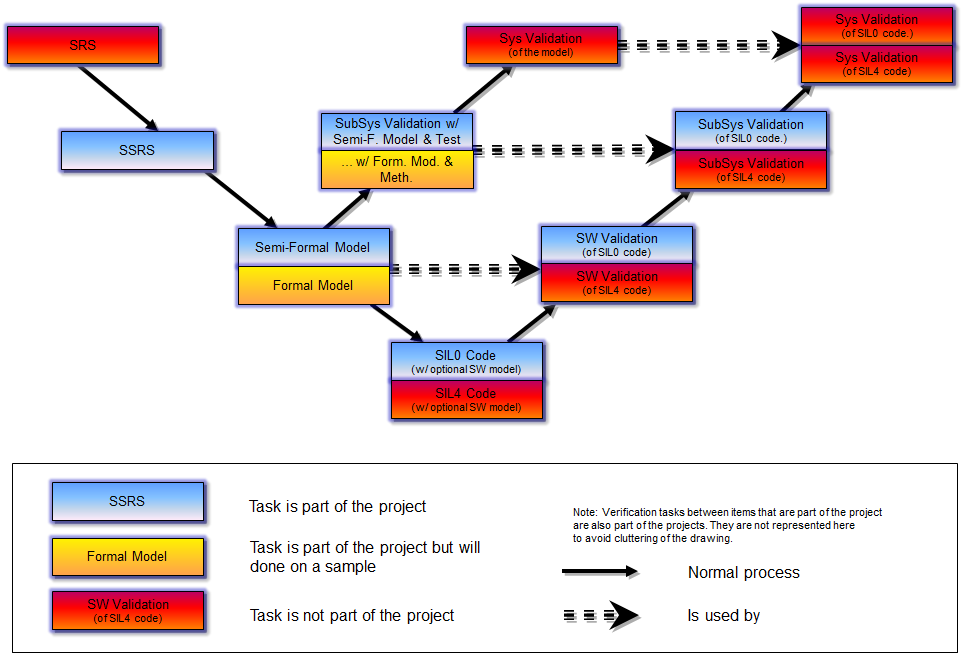
\includegraphics[scale=0.65]{Process1.png}}
  \caption{Main process}
  \label{fig:main_process}
\end{figure}
 
 
It starts by the SRS which is not part of the project (SUBSET-26), then outlines the boundaries and 
the applicable requirements from the SUBSET-26 that will be used in the formal model. This step  is described in EN50129  as system development phase.

The next step is the creation of the formal model itself. Because this model is executable, it can 
be validated as itself, thus the first ``closing branch'' of the V.
This step has to been linked with the following phases described in EN50128 :
\begin{itemize}
\item Software requirement
\item Software architecture and design
\item Software component design
\end{itemize}

From the model can be derived some ``abstract'' code. The word ``abstract'' is used to emphasize that 
this code is not necessarily capable of running of a full SIL4 platform. This code can be validated 
in the second ``closing branch'', possibly using some of the work done in the first branch. 
This step  is described as software component implementation design in EN50128.

A project demonstrator may be derived from this code (or may be the ``abstract'' code itself).

The third ``closing branch'' corresponds to the production of code capable of running on a 
given SIL4 platform, and the associated validation activities. This is not part of the project.

The yellow boxes corresponds to activities that should be covered completely in order to produce 
a certifiable product, but of which only a subset will be conducted in order to demonstrate the 
capabilities of the product.

 
Fig. \ref{fig:safety_process} shows activities that are needed for the safety analyses. It should 
be considered in parallel of the descending branch of the V, but has been put on a separate diagram for
the sake of clarity.

High level safety properties are provided, which must be refined side-to-side with each step on the 
descending branch of the V. These properties are then used for the safety analysis of the model. The 
validation (safety analyses) boxes are yellow because the full activity will not be conducted. Only 
a subset of the safety properties will be proved.

\begin{figure}
  \centering
  \fbox{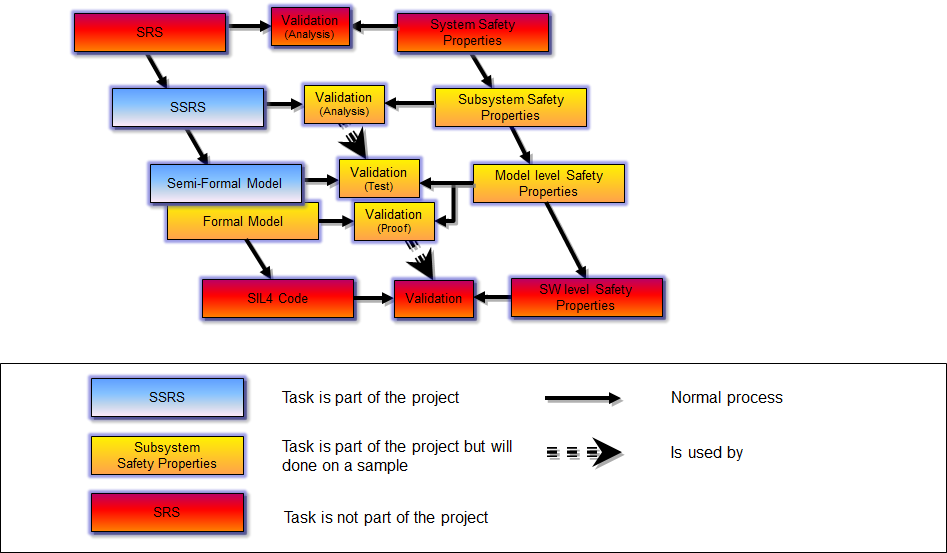
\includegraphics[scale=0.80]{Process2.png}}
  \caption{Safety analyses}
  \label{fig:safety_process}
\end{figure}



The proposed process shall comply the CENELEC standard EN 50126, EN 50128  and EN50129, expecially the proposed lifecycle of \ref{fig:develop-lifecycle-cenelec}.


\begin{figure}[ht]
  \centering
  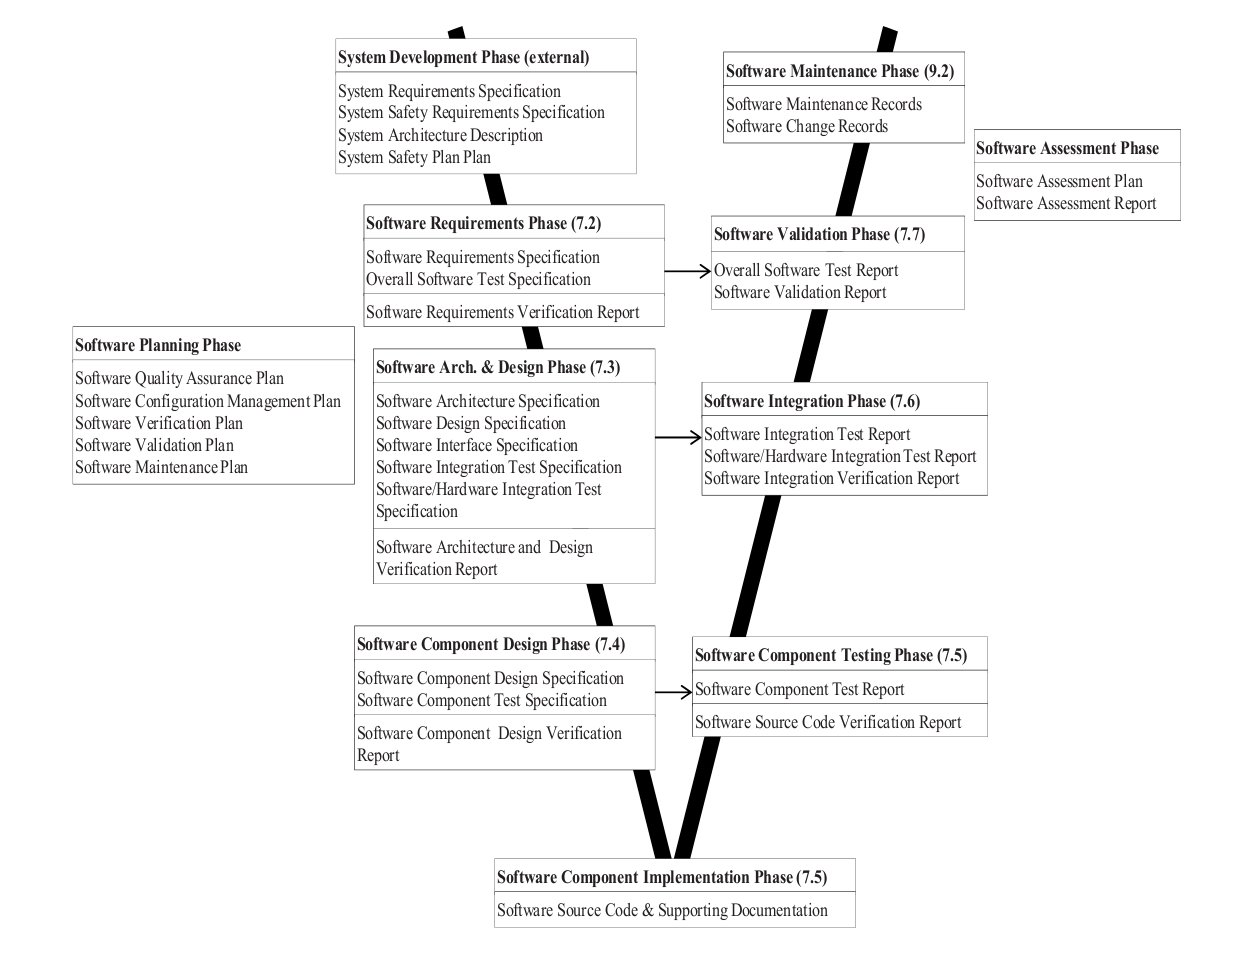
\includegraphics[width=\textwidth]{V-Model}
  \caption{General Development Lifecycle~\cite{EN-50128}}
  \label{fig:develop-lifecycle-cenelec}
\end{figure}


 It consists of the SW planning phase in the beginning, the SW assessment phase at
the end and the following development phases:

\begin{itemize}
\item System Development Phase
\item SW Development Phases
  \begin{itemize}
  \item SW Requirements Phase
  \item SW Architecture and Design Phase
  \item SW Component Design Phase
  \item SW Component Implementation Phase
  \end{itemize}
\item SW Test / Validation Phases
  \begin{itemize}
  \item SW Validation Phase
  \item SW Integration Phase
  \item SW Component Testing Phase
  \end{itemize}
\end{itemize}

Software planning phase is defined by WP1 in the Quality Assurance Plan.
Software Test / Validation phase is defined by WP4 in Validation Plan.
Software Verification activities are defined by WP4 in Verification Plan.

Safety activities are described in EN50126.
However proof that the process satisfies the requirements of the standard is out of the scope of this document and shall be manage by the Safety Case (WP4).





\subsection{System Development Phase}
\label{sec:syst-devel-phase}

\todo{To develop}
\begin{comment}This section shall define the activities links to  the system specification and model. 

This step is not explicitly defined in EN 50128 but is defined in EN 50129. However EN 50128  gives the expected output from this step  for the software activities :  System  Requirements Specification, System Safety Requirements Specification, System Architecture Description, External  Interface Specifications
\end{comment}

\begin{issue}
To discuss with all partners :  Do we need a SSRS ? This is expected by EN50129.

S. Baro comments (15/02/2013) :

SSRS

We had a un-conclusive discussion on the necessity to insert a SubSystem Requirement Specification betwen the SRS (subset 26) and the formal model. The reason of this is that the model we want corresponds to a subsystem (part of the OBU), but the SRS corresponds to the whole system. The SRS also does not provide any functional architecture, and we think it is necessary to provide one. In the other hand, it adds one document between the SRS and the model. The question is thus to know if this document will remove more errors than it will add.
Proposal: To provide a SSRS which contains:
- a formal or semi-formal functional architecture of the OBU part which will be modeled, with function "boxes" and I/O "arrows";
- the requirements allocated to the functions and I/O, rewritten but still in natural language;
- the tagging Safety/Non Safety of these requirements.
This document should be seen as an important step of the modeling process, and would be under the responsibility of WP3.
 

\end{issue}

\paragraph{Objectives:}
\label{sec:sys-dev-objective}
The aim of this phase is to have a clear definition of the system to design :

\begin{itemize}
\item a set of system requirements which discribe the functionality of the system as the expected results concerning performance, maintenability, safety, fiability,...
\item the description of the architecture of the system 
\item interface descriptions
\end{itemize}


Safety activities are necessary to define the safety requirements of the system and to defined which functions are tagged Vital or Non-Vital.

\paragraph{Documents:}
\label{sec:sys-dev-documents}
The documents to produce in this phase are :
\begin{itemize}
\item the system safety plan explains the overall
approach to ensure safety in the developed system
\item the system requirements
specification describes all requirements of the system
\item the system safety requirements
specification focusses on the safety aspects
\item the system architecture specification
and SW / HW interface definition which specify how the SW and the HW interact
and the location of the boundary between the two
\end{itemize} 

\paragraph{Detailed Description:}
\label{sec:sys-dev-deta-descr}
Figure~\ref{fig:detailed-sys-dev-phase} describes an iteration in this phase in
more detail.

\begin{figure}[ht]
  \centering
  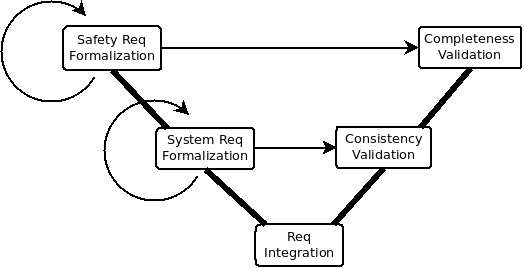
\includegraphics[width=.5\textwidth]{System-Dev-Phase-Details}
  \caption{Sub Process in System Development Phase}
  \label{fig:detailed-sys-dev-phase}
\end{figure}

The first phase is the formalization of the safety requirements, this it
iterated until internal consistency is ensured. The next phase is the
formalization of the system requirements, analogously with an iteration to
ensure their consistency.

Both sets of requirements are combined in the requirement integration
phase. They shall be transformed into a common formal specification format if
necessary. The consistency of the combination is verified in the next phase and
finally the completeness of the requirement wrt. informal specification. Any
deviation from the consistency of the combined requirements or from the
completeness shall be documented and the phases reiterated until consistency and
completeness is achieved.


\begin{comment} Some requirements to take into account :
\end{comment}

\req{The model shall be consistent with the SRS level and shall yield as
few as possible “design choices”.}
\subreq{Traceability with the SRS shall be provided. }
\subreq{Each interpretation of the SRS shall be indicated precisely.}
\subreq{Each SRS requirement not formalized in the model (\emph{e.g.} allocated to RBC)
should be traced and justified.}



\req{When the boundary of the formalized subsystem corresponds to a FIS or FFFIS, the Functional 
Architecture shall try to comply to it even when it is not mandatory.}

\req{The Functional Architecture shall split the KERNEL into independent functions.}

\req{The Functional Architecture shall identify a subset of these functions that will be modeled.}
\req{The Functional Architecture shall allow a universal method of adding function (modularity).}



\subsection{Model definition}
\label{sec:sw-development-phase}

\subsubsection{SW Requirements Phase}
\label{sec:sw-requ-phase}

\todo{To  detail according § 7.2 of EN 50128}

\paragraph{Objectives:}
\label{sec:sw-req-objective}


In this phase, the system requirements shall be declined to take into account software constraints.

In particular software requirements specification shall give a description of all the input/output of the software, a description of the operational modes and behaviour. It shall provides all the element to have testable requirements. All function to perform shall be clearly identify. All existing constraints of the
constraints between HW and SW will be taken into account (cf. §7.2.1.1).



\paragraph{Documents:}
\label{sec:sw-req-documents}
The documents to produce in this phase are :

\begin{itemize}
\item the SW requirements specification
\item the overall SW testing specification will provide the detailed approach
to test the developed SW, concretizing the approach in the SW testing plan
\item the SW requirements verification report will document the results
of the verification of the SW requirements specification wrt. the criteria
specified in §7.2.4.22 (cf. §7.2.3).
\end{itemize} 

\paragraph{Responsible:}
\label{sec:sw-req-responsible}
RQM

\paragraph{Detailed Description:}
\label{sec:sw-req-deta-descr}

\tbc

%For the overall SW test specification the use of modeling is recommended
%(cf. A.7) and for this formal methods are one of the highly recommended methods
%(cf. A.17), , a formal model for model-based testing can be part of the
%overall SW test specification.
%
%Figure~\ref{fig:detailed-sw-dev-phase} shows the proposed sub-phases of the SW
%requirements phase.
%
%\begin{figure}[ht]
%  \centering
%  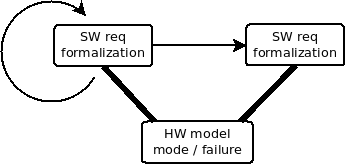
\includegraphics[width=.35\textwidth]{SW-Req-Phase-Details}
%  \caption{Sub Process in SW Development Phase}
%  \label{fig:detailed-sw-dev-phase}
%\end{figure}
%
%The first phase consists of the description and formalization of the SW
%requirements. The system architecture model from the preceding phase shall be
%extended with a model of the SW. All SW requirements shall be referenced in that
%model. The internal consistency of the SW requirements shall be verified with an
%appropriate formal verification tool, any inconsistency shall be
%documented. This shall be iterated until consistency of the SW requirements is
%achieved.
%
%In the next phase a formal behavioral model of the programmable electronic HW is
%produced which includes in particular the desired behavior in case of
%failures.
%
%The SW requirements together with the HW model are combined in an appropriate
%formal specification  and the consistency and correctness wrt. the system
%requirements and the safety requirements shall be verified formally. The
%deviations shall be documented. They shall be fixed in the next in-phase
%iteration.
%



\subsubsection{SW Architecture and Design Phase}
\label{sec:sw-arch-design}

\todo{To  detail according § 7.3 of EN 50128}

\paragraph{Objectives:}
\label{sec:sw-arch-objectives}
In this phase a SW architecture shall be developed which allows to meet the SW
requirements and the necessary safety requirements without introducing
unnecessary complexity. In this phase there shall also be an evaluation of the
HW / SW interaction, its influence on the safety aspects of the system and the
valuation of the usage of already existing SW. It shall also ensure the
testability and the appropriateness for formal proofs of the resulting SW, in
particular by minimizing the complexity and the size of the safety relevant
parts (cf. §7.3.1.1 to 7.3.1.5).



\paragraph{Documents:}
\label{sec:sw-arch-documents}
In this phase the following documents shall be produced: 
\begin{itemize}
\item the
specifications for the SW architecture
\item the SW design and the SW interface
\item the specification for the SW integration test and for the SW
/ HW integration test
\item the SW architecture and design verification
report will document whether this phase has been finished in accordance with
the standard (cf. §7.3.3)
\end{itemize} 

\paragraph{Responsible:}
\label{sec:sw-arch-responsible}
DES, VER, INT

\paragraph{Detailed Description:}
\label{sec:sw-arch-deta-descr}
The details of the sub-process of the SW architecture and design phase is shown
in Figure~\ref{fig:detailed-sw-arch-phase}.

\begin{figure}[ht]
  \centering
  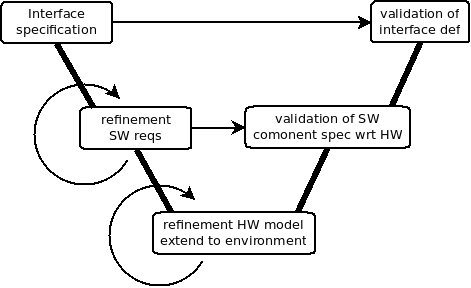
\includegraphics[width=.5\textwidth]{SW-Arch-Phase-Details}
  \caption{Sub Process in SW Architecture and Design Phase}
  \label{fig:detailed-sw-arch-phase}
\end{figure}

\tbc 

%In the first phase the interfaces of the SW to other SW and to HW shall be
%formally defined in an appropriate specification language. In particular the
%necessary pre- and postconditions, used parameters and their boundaries shall be
%described in a formal way~\footnote{ in ACSL~\cite{baudin09acsl} the
%  annotation language used by Frama-C (\url{http://frama-c.com})}
%
%The next step is to refine the SW architecture to components. The SW
%requirements specification shall be refined to these components. It shall be
%formally verified that the requirements of the components are internally
%consistent and that they are correct wrt. SW requirements specification. Any
%found deviation shall be documented and the sub-phase shall be iterated until
%consistency and correctness is achieved.
%
%The model of the programmable HW shall be further refined and be extended with a
%formal description of the system into which the SW will be integrated. This
%model shall be verified wrt. safety requirements, any deviation shall be
%documented and fixed for a later iteration of this sub-phase.
%
%The consistency of the SW component requirements specification wrt. the HW
%behavioral model shall be verified, as well as the consistency of the interface
%definition wrt. SW components and the HW parts of the system. Deviations shall
%be recorded and the sub-phase shall be iterated until consistency is reached.


\subsubsection{Software Component Design Phase}
\label{sec:softw-comp-design}
\todo{To  detail according § 7.4 of EN 50128}

\paragraph{Objectives:}
\label{sec:sw-comp-objectives}
This phase shall develop a low level specification for each of the SW components
which is correct wrt. requirements of the SW design specification and of the SW
component design specification (cf. §7.4.1.1, §7.4.1.2).


\paragraph{Documents:}
\label{sec:sw-comp-documents}
\tbc

\paragraph{Responsible:}
\label{sec:sw-comp-responsible}
DES, VER

\paragraph{Detailed Description:}
\label{sec:sw-comp-deta-descr}

\tbc


%This phase shall replace the manual steps component implementation and component
%testing with unit-tests which are present in the original development
%lifecycle. The formal proofs will ensure correctness of the generated code
%wrt. specification, therefore making testing superfluous. The outline of this is
%shown in Figure~\ref{fig:proof-code-generation}, where the green arrow marks the
%proposed ``shortcut''. According to the standard, such an approach and the
%applied tools must be appropriate according to 6.7.4.4.
%
%\begin{figure}[ht]
%  \centering
%  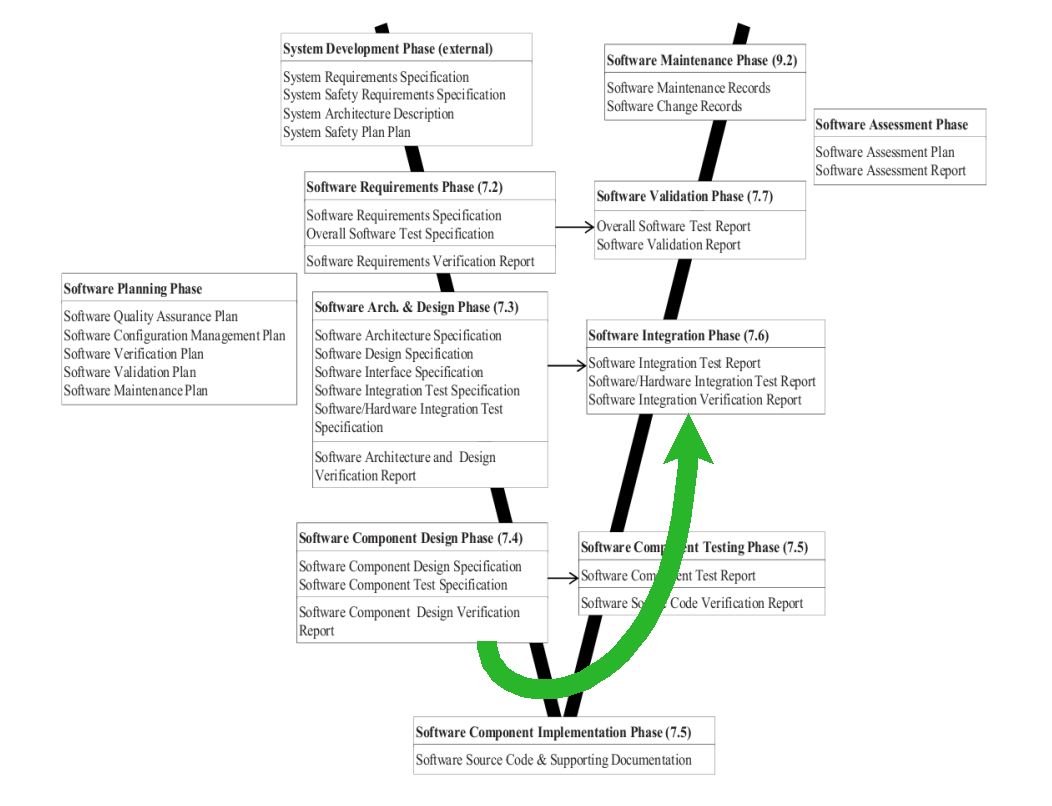
\includegraphics[width=\textwidth]{V-Model-abk}
%  \caption{Formal Proof and Automatic Code Generation in V-Model}
%  \label{fig:proof-code-generation}
%\end{figure}
%
%The sub process in this phase is shown in
%Figure~\ref{fig:detailed-sw-comp-phase}.
%
%\begin{figure}[ht]
%  \centering
%  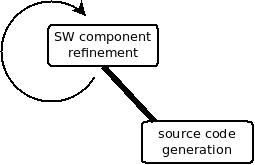
\includegraphics[width=.3\textwidth]{SW-Comp-Phase-Details}
%  \caption{Sub Process in SW Component Design Phase}
%  \label{fig:detailed-sw-comp-phase}
%\end{figure}
%
%The SW component refinement phase shall verify the correctness of the refinement
%wrt. the SW component requirements specification. This sub-phase shall be
%iterated until the specification of the behavior of each SW component is
%detailed enough to be eligible to automatic code generation. A suitable
%formalism for this approach shall be a formal framework which supports formal
%proofs of properties, supports iterative refinement, supports refinement proofs
%and is suitable wrt. criteria of the standard\footnote{ the Event-B method
%  as integrated int the Rodin tool~\cite{Abrial:Rodin}
%  (\url{http://www.event-b.org/})}. Finally the source code shall be generated
%from the formal behavior specification.
%
%Although automatically generated, the source code shall contain annotations for
%the pre- and postconditions and other properties,  loop invariants. The
%generated code shall also adhere to the coding standards of as defined in the SW
%design specification. This will ensure that the generated code is human readable
%and facilitate its potential re-use in other projects.



\subsection{Abstract Code}

\todo{To  detail according § 7.5 of EN 50128}


\subsubsection{Software Component Implementation Phase}
\label{sec:softw-comp-impl}

\tbc

\begin{issue}
Manual versus automatic code generation ?
\end{issue}
Shall be replaced by automatic code generation from formal models using
refinement techniques.

\subsubsection{Software Component Testing Phase}
\label{sec:softw-comp-test}

\begin{issue}
Verification step ?
\end{issue}

\subsubsection{Software Integration Phase}
\label{sec:softw-integr-phase}

\begin{issue}
Verification or validation step ?
\end{issue}

%\paragraph{Objectives:}
%\label{sec:sw-int-objectives}
%This phase shall demonstrate the correct functioning of the combination of the
%developed SW components, in particular in their target HW environment. The
%necessary tests for this phase are specified in the SW / HW integration test
%specification and SW integration test specification (cf. §7.6.1.1, §7.6.1.2).
%
%\paragraph{Formal Methods:}
%\label{sec:sw-int-formal-methods}
%Any deviation which is found in this phase shall be documented. The results of
%this phase shall be used to refine the formal models if necessary, in particular
%the formal models of the HW.
%
%\paragraph{Documents:}
%\label{sec:sw-int-documents}
%The SW integration test report shall document the results from the integration
%of the SW, the SW / HW integration report the results from the integration of
%the developed SW on the target HW. Both shall include the test cases, their
%respective results and document all details of the configuration for the
%tests. The SW integration verification report shall document whether the test
%reports have been written according to their respective specifications and
%adhere to the relevant parts of the standard for test reports (cf. §7.6.3).
%
%\paragraph{Responsible:}
%\label{sec:sw-int-responsible}
%INT, VER
%




\subsection{Safety activities}

\todo{this activity is not explicitly detailed in 50128 (except some task  in different activities)  but in 50126 and 50129 }

\begin{comment} from D.2.{6,7,8,9} : 
\end{comment}

\begin{justif}
Side to side with the model (which should be a dynamic model), should lay a set of  
static safety properties on the model. The higher level properties will be provided 
by the WP2 (equivalent to a preliminary hazard analysis) from the SUBSET-91 document, 

They will be refined by the safety analysis process (WP4) into properties of the same 
level than the model. The process of doing so shall be described in the Safety Plan.

This will provide Safety Properties on the model (or Dread Events). The lower level Safety Properties/
Dread Events shall address variables, state and interfaces used in the formal model.

Formal proof would then be used to prove that the OpenETCS model never enter a Dread State, 
as long as the other subsystem (RBC, communication layer\dots) fulfill their own safety properties
(axiom describing the environment).
\end{justif}

\req{A safety plan shall be provided and complied with.}
\req{The Functional Architecture shall identify the Vital and Non Vital functions.}
\begin{comment}
MPD : Identification of Vital and non vital  can be done only if the safety  analysers have provided safety properties and have allocated them to  functions.
\end{comment}
\req{The subsystem shall be compatible with the THR required in the SUBSET-091.}
\req{The safety analysis shall consider the Dread Event of the SUBSET-091, restricted to the
scope of the subsystem.}
\req{The model-level safety properties shall be written in a formal language.}

\begin{issue}
To discuss with all partners :  what is expected on this activity in the process.

S. Baro comments (15/02/2013) :

Safety

Are safety activities required in this project? The project require "certifiability" of some items (toolchain? model?) and compliance to 50128. For the toolchain, it is quite clear what it means, but for the model it is much more complicated. Is it really required for the model? If safety activities are required on the model, I think it makes no sense to refer only to 50128: it should refer to 50126 and 50129 too (excluding the hardware part which is not in the scope of the project). This pulls system safety analysis, safety properties,... but provides the initial properties required for formal proof on the model (once refined through system safety analysis).
Proposal: The "Safety" WP provides a safety case concept and safety plan according to Merlin's document and to the requirements. It is not realistic to expect that the full safety case will be provided for OpenETCS, but I think it will be useful to conduct a sample of the tasks, or all tasks but on a sample of the model. The higher level properties will be provided by subset 91, and refined by the safety analysis to properties on the model (I provided an example on how to do this in another document). Please note that even covering the whole subset 91 properties is certainly not sufficient to ensure the safety of the model.
Question: who will provide the manpower for safety activities? WP4? 

\end{issue}


\subsection{Verification and Validation}

Each of the SW development phases shall have an appropriate test / validation
counterpart, as illustrated in the V form of the lifecycle. 


The Verification and Validation activities have to be planned on the whole process according the requirement of EN50128 § 6.2 and 6.3.

This plan is out of the scope of the document and shall be defined in the WP4 process.

\todo{To check the existing draft on this subject}

%\subsubsection{Overall Testing / Final Validation}
%\label{sec:overall-testing-}
%
%\paragraph{Objectives:}
%\label{sec:sw-test-objectives}
%The objective of this phase is to validate the adequacy of the developed SW and
%its integration wrt. system requirements specification, the functional
%properties and the safety related properties of the system according to the
%SIL. In this phase the overall fitness for purpose of the system will be
%evaluated (cf. §7.7.1.1).
%
%\paragraph{Formal Methods:}
%\label{sec:sw-test-formal-methods}
%This phase is executed by the VAL who will validate the developed system. In
%particular, he will analyze whether the chosen combination of techniques are
%appropriate wrt. standard,  the use of formal proofs in
%phase~\ref{sec:softw-comp-design} to replace phases~\ref{sec:softw-comp-impl}
%and~\ref{sec:softw-comp-test}.
%
%\paragraph{Documents:}
%\label{sec:sw-test-documents}
%The VAL will produce the overall SW test report in which the VAL will document
%the results of additional tests he specified and executes himself or lets TST
%execute them. The VAL will also produce a SW validation report which shall
%document the results of the SW validation plan. The VAL will also produce a
%release note which shall document any restriction of the usage of the developed
%software (cf. §7.7.3).
%
%\paragraph{Responsible:}
%\label{sec:sw-test-responsible}
%VAL

